% ============================================================
%  Report Template
% ============================================================

\documentclass[11pt]{article}

% ── Packages ────────────────────────────────────────────────
\usepackage[margin=1in]{geometry}
\usepackage{amsmath, amssymb, amsthm}
\usepackage{booktabs}
\usepackage{graphicx}
\usepackage{hyperref}
\usepackage{natbib}
\usepackage{setspace}
\usepackage{microtype}
\usepackage{enumitem}
\usepackage{caption}
\usepackage{subcaption}
\usepackage{xcolor}
\usepackage{float}
% code packages
\usepackage{listings}
\usepackage{inconsolata}
\lstset{basicstyle=\ttfamily\footnotesize,breaklines=true}
\usepackage{csvsimple}
\usepackage{booktabs}

% ── Hyperref setup ──────────────────────────────────────────
\hypersetup{
    colorlinks = true,
    linkcolor  = black,
    citecolor  = black,
    urlcolor   = blue
}

% ── Theorem environments ────────────────────────────────────
\newtheorem{theorem}{Theorem}
\newtheorem{proposition}{Proposition}
\newtheorem{lemma}{Lemma}
\newtheorem{corollary}{Corollary}
\theoremstyle{definition}
\newtheorem{definition}{Definition}
\newtheorem{assumption}{Assumption}
\theoremstyle{remark}
\newtheorem{remark}{Remark}

% ── Spacing ─────────────────────────────────────────────────
\onehalfspacing

% ── Title block ─────────────────────────────────────────────
\title{Problem Set 1}
\author{Tate Mason}
\date{\today}

% ============================================================
\begin{document}
\maketitle
\thispagestyle{empty}

% ── Abstract ────────────────────────────────────────────────

\newpage
\setcounter{page}{1}

% ── 1. Introduction ─────────────────────────────────────────
\section{Introduction}

Through this problem set, we were able to gain practical experience in differences between pricing regimes, and the efficacy of zone pricing.
Following the work of Adams and Williams (2019) and Dellavigna and Gentzkow (2018), we will use simulated data on Walmart and Target. In the first
problem, data facts will be presented, pointing out some interesting findings, as well as market level profits for both firms. Then, in the second,
estimation results will be reported for OLS, 2SLS, and BLP methods. Finally, the final problem will take a closer look at the pricing regimes, presenting
a best response table as well as consumer surplus under each permutation.

% ── 2. Data Facts ─────────────────────────────────────────────────
\section{Data Facts}

\subsection{Income Sorting}

First, I would like to present a histogram of the distribution of market activity for each firm. For all plots, Walmart will be the blue firm and Target the red.

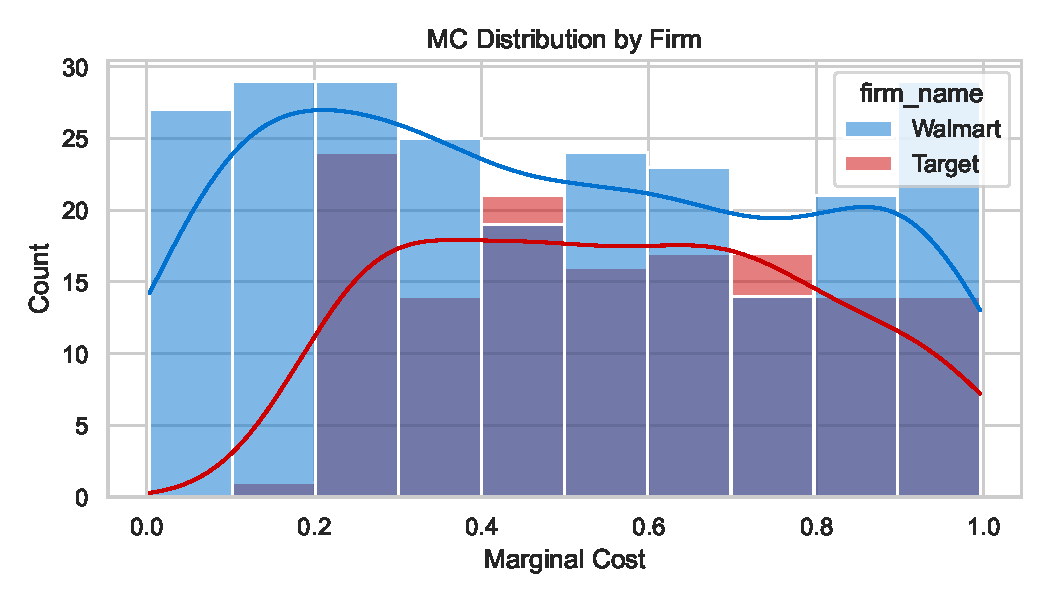
\includegraphics{../Graphics/mc_dist.pdf}

Walmart is able to run more cheaply, but with much more dispersion. Most of their firms are the low end of the marginal cost distribution, before tapering down. 
Target, however, is relatively stable between the 0.4-1.0 marginal cost buckets. Notice, however, Walmart is still more abundant across the entire cost distribution,
save for two buckets.

\subsection{Income Structure}

Next I will present the distribution of income across the markets. This is important, as it will allow us to understand the heterogeneity in the consumer base, and how that may affect the pricing decisions of the firms.

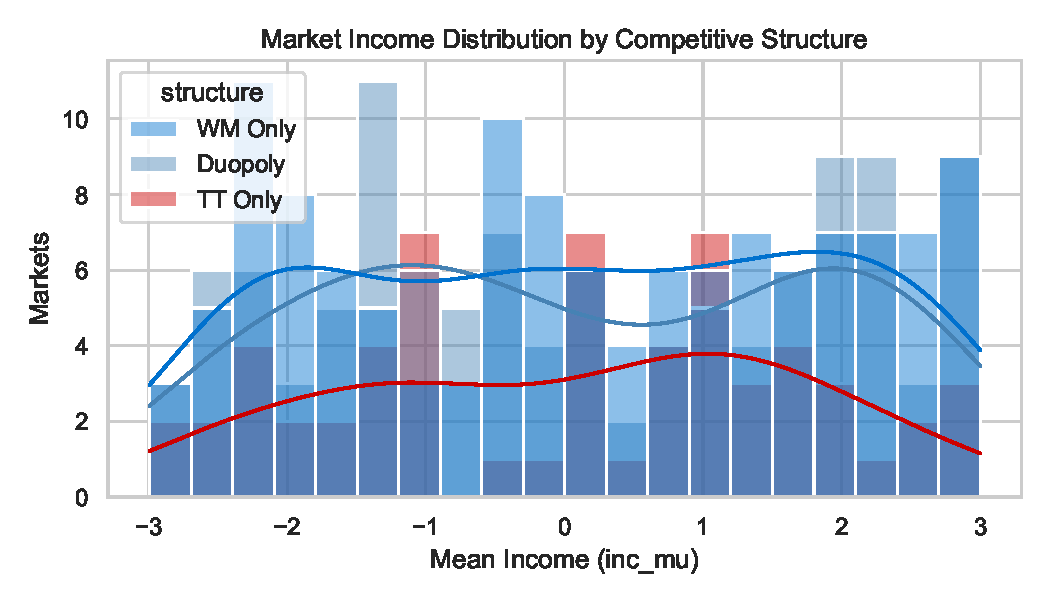
\includegraphics{../Graphics/income_structure.pdf}

I will break this down in the three categories: only Walmart, only Target, and both. There are many more only Walmart markets across the entire mean income distribution. In fact, there are more only Walmart markets than markets with both firms as well,
which is interesting. Target, on the other hand, is much less likely to be the only firm in a market, seeming to focus mostly on markets between -1 and 1 in mean income. The both category is closely linked with Walmart, a fact easily seen from the fit line. 
It would seem that income does not tell a ton.

\subsection{Variety and Share}

I was also curious is the variety in product characteristics had any relationship with the share of the market. 

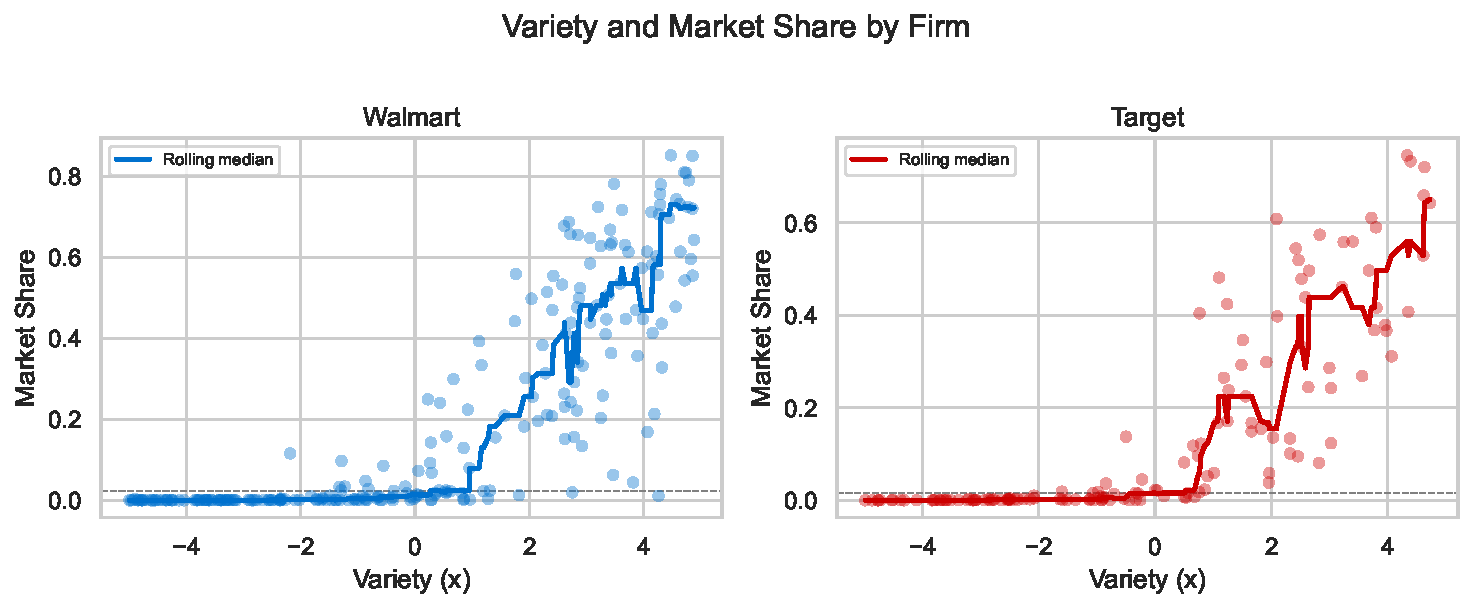
\includegraphics[width=\textwidth]{../Graphics/variety_share.pdf}

Here, there is a positive relationship for both firms, but Walmart exhibits a much clearer trend, whereas Target has more noise. This indicates that Walmart is more likely to carry more varied products, while Target may specialize more.

\subsection{Markup Distribution}

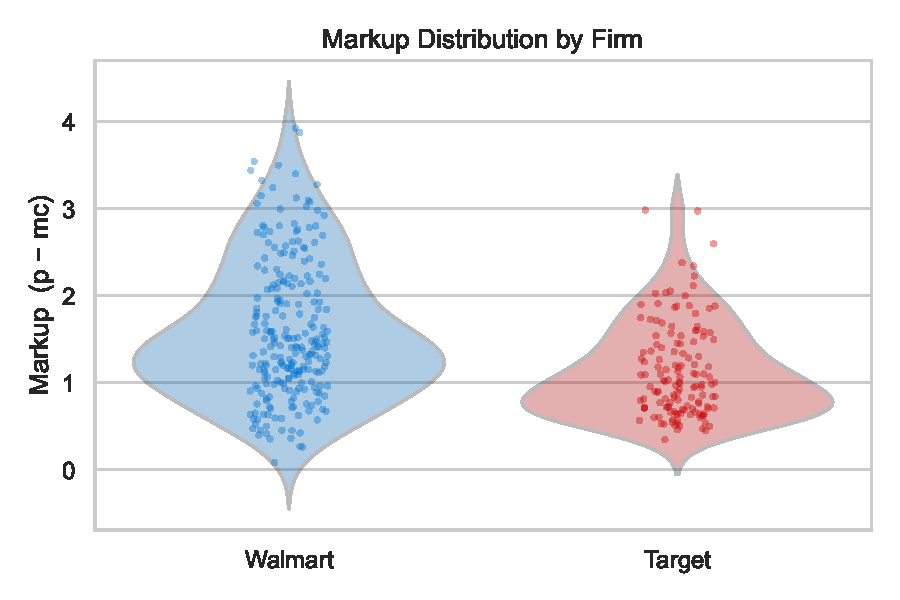
\includegraphics{../Graphics/markup_dist.pdf}

Markups are much more condensed for Target, with most of the markups between 0.5-2. Walmart, contrastingly, is much more dispersed, with mass spread between 0.25-4. This is interesting, as it points to Target having more control over their pricing and costs, while Walmart is more volatile.
This could be due to the wide spread of marekts that Walmart serves, leading to evidence of monopoly power in some markets, and more competitive pressure in others.

\subsection{Prices}

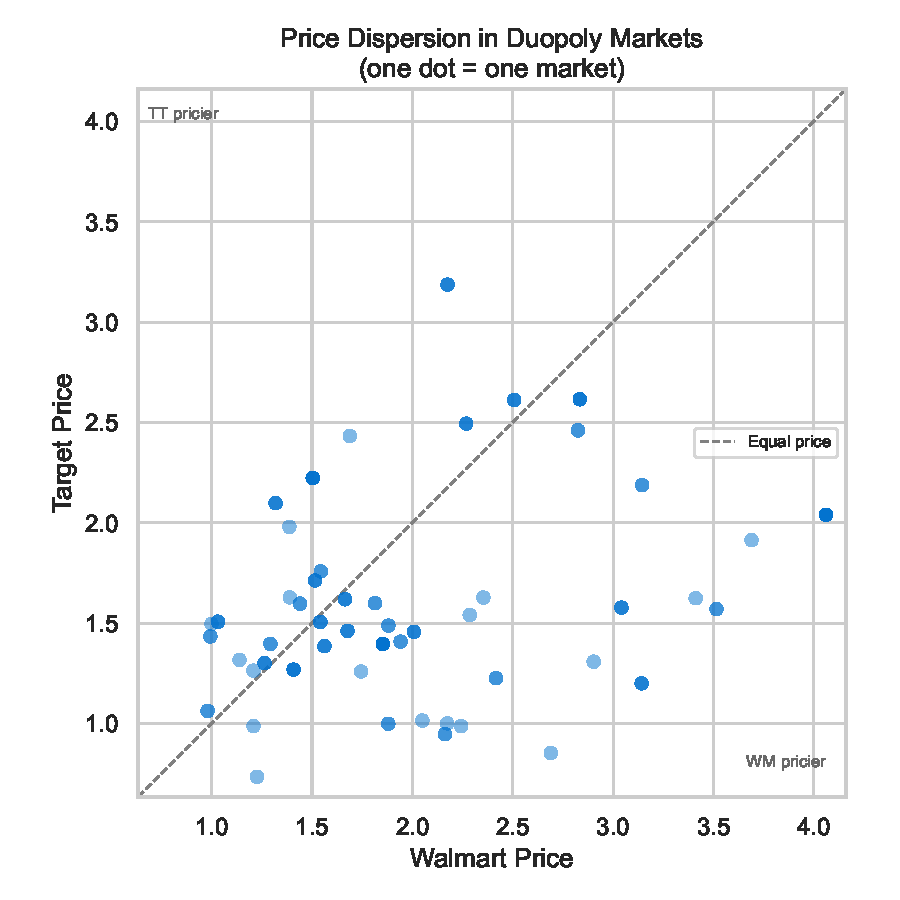
\includegraphics{../Graphics/price_dispersion.pdf}

This figure shows price competitions in duopoly markets. Walmart prices higher in a majority of the markets, and when Target does exert pricing power, they are closer to the competitive line than Walmart's deviations. This again points to Walmart having more market power, and in fact may point to zone pricing behavior.

\section{Profits Table}

\begin{table}[H]
    \centering
    \caption{Profits by Market}
    \label{tab:profits}
    \csvautobooktabular{../Data/profits_summary.csv}
\end{table}

Here, we can see that Walmart has higher profits as well as higher variance in profits. This is interesting, as it affirms the idea that Walmart is more likely to have market power in many markets, but it must compete in the markets where Target is present. Target's mean profits are almost half that of Walmart. The variance is also lower, but still very high given the mean. 
Even looking at the max profits, Walmart is able to max out at 150\% that of Target, another indication that Walmart is much more able to exert market power.

A full csv of profits by markets is included in the data folder, but I shortened to the summery for the sake of presentation.

\subsection{Data Facts Conclusion}

It would appear from these figures that Walmart is more likely to have the market power advantage, either through monopoly or in competitive markets. Target, on the other hand, seems to be more of a niche player, staying in its lane with pricing and markups. These facts are interesting due to Target's reputation as a 
more upscale retailer. However, it would seem that Walmart is able to leeverage its size and scale to compete on its own terms, and thus is able to exert more market power in a majority of the provided markets.

% ── 3. Model / Theoretical Framework ───────────────────────
\section{Model and Estimations}

In this section, I will present estimation results and brief interpretations of said reults. We will
begin by reporting OLS results, before moving into 2SLS, and finally a BLP GMM procedure.

\subsection{OLS}

We first undertake a simple OLS, regressing the log difference between own and outside share on characteristics, price, and a constant.

\begin{gather*}
  \log{(s_j - s_0)} = \beta_0 + \beta_jx_j + \alpha_jp_j \\
  \text{such that} \\
  s_0 = 1 - \sum_{k\ne j}s_k
\end{gather*}

\begin{table}
\centering
\begin{tabular}{lcc}
\toprule
  & Parameter & Std. Error \\
\midrule
  Const. & -2.42 & 0.21 \\
  Characteristics & 1.26 & 0.03 \\
  Price & -0.91 & 0.10 \\
\bottomrule
\end{tabular}
\caption{OLS Estimates}
\end{table}

Going off of the true parameters, we can see the OLS estimates are biased away from zero.
This is to be expected, as price is an endogenous variable, thus OLS is not going to produce
a consistent estimate.

\subsection{2SLS}

Next, I will present the 2SLS estimates, using the marginal cost as an instrument for price.

\begin{gather*}
  \log{(s_j - s_0)} = \beta_0 + \beta_jx_j + \alpha_jp_j \\
  p_j = \pi_0 + \pi_jx_j + \gamma_jmc_j
\end{gather*}

\begin{table}
\centering
\begin{tabular}{lcc}
\toprule
  & Parameter & Std. Error \\
\midrule
  Const. & -0.48 & 2.935 \\
  Characteristics & 1.26 & 0.03 \\
  Price & -1.92 & 1.52 \\
\bottomrule
\end{tabular}
\caption{2SLS Estimates}
\end{table}

These estimates bias still bias $\alpha$ away from zero, but less than OLS. This is to be expected, since the MC instrument is weak, but still picks 
up some the variation. The standard error is also much higher, which is also expected, as the instrument is weak. The characteristics parameter is unaffected, as it is exogenous.

\subsection{BLP}

Finally, I will present the BLP GMM estimates, which should be the most consistent of the three. I will continue to instrument for price as in 2SLS, but will also
include the interaction of characteristics and income, as well as income and MC. This will allow me to parse out the heterogeneity due to income.

\begin{table}
\centering
\begin{tabular}{lcc}
\toprule
  & Parameter & Std. Error \\
\midrule
  Const. & -1.37 &  2.51 \\
  Characteristics & 1.21 & 0.06 \\
  Price & -1.80 &  1.36 \\
  Char. x Income & 0.07 & 0.00 \\
  Income x MC & 0.32 & 0.00 \\
\bottomrule
\end{tabular}
\caption{BLP Estimates}
\end{table}

My estimates are for the most part close to the true parameters set during the DGP.
Only $\alpha_i$ is still pretty far, but the instruments are still weak, so I am not
surprised.

% ── 4. Empirical Strategy ───────────────────────────────────
\section{Regime Comparison}

This section will discuss the different pricing regimes, and what the best response is for each firm. First, however, I will 
briefly derive the FOC's for the firms, which will then be used in my functions to calculate the profits under each regime.

\subsection{FOC's}

\textbf{Uniform Pricing:} Under uniform pricing, the firms set a single price for all consumers.

\begin{gather*}
  \pi_j = \sum_t 1000*(p_j - c_j) \cdot s_j \\
  \frac{\partial \pi_j}{\partial p_j} = s_j + (p_j - c_j) \cdot \frac{\partial s_j}{\partial p_j} = 0 \\
  \text{which implies} \\
  p_j = c_j - \frac{s_j}{\frac{\partial s_j}{\partial p_j}}
\end{gather*}

\textbf{Zone Pricing:} Under zone pricing, the firms can set prices which span zones depending on the market power of the firm in the two zones.

\begin{gather*}
  \pi_{jz} = \sum_{t\in Z} 1000*(p_{jz} - c_{jt}) \cdot s_{jt} \\
  \frac{\partial \pi_j}{\partial p_{jz}} = \sum_{t\in Z} s_{jt} + (p_{jz} - c_{jt}) \cdot \frac{\partial s_{jt}}{\partial p_{jz}} = 0 \\
  \text{which implies} \\
  p_{jz} = \frac{\sum_{t\in Z} \frac{\partial s_{jt}}{\partial p_{jz}} \cdot c_{jt} - s_{jt}}{\sum_{t\in Z} \frac{\partial s_{jt}}{\partial p_{jz}}}
\end{gather*}

\textbf{Market Pricing:} Under market pricing, the firms can set prices for each market, thus maximizing profits in each market.

\begin{gather*}
  \pi_{jt} = 1000*(p_{jt} - c_{jt}) \cdot s_{jt} \\
  \frac{\partial \pi_{jt}}{\partial p_{jt}} = s_{jt} + (p_{jt} - c_{jt}) \cdot \frac{\partial s_{jt}}{\partial p_{jt}} = 0 \\
  \text{which implies} \\
  p_{jt} = \frac{\partial s_{jt}}{\partial p_{jt}} \cdot s_{jt} - c_{jt}
\end{gather*}

Note: $\frac{\partial s_{jt}}{\partial p_{jz}} = \alpha s_{jt}(1-s_{jt})$ with only notation differences between the regimes.

\subsection{Best Response Table}
\begin{table}
\centering
\begin{tabular}{lccc}
\toprule
  & Uniform & Zone & Market\\
\midrule
  Uniform & (49955, 15402) & (42160,15911) & (39247, 16151) \\
  Zone & (50809, 11500) & (42709, 11935) & (39755, 12178) \\
  Market & (51269, 9796) & (42871, 10114) & (39874, 10395) \\
\bottomrule
\end{tabular}
\caption{Best Response Table}
\end{table}

From the table, I will concede I have made a mistake. Walmart should not want to choose unifrom, as it can exert any pricing regime due to Target's lack of 
market power. So, Walmart should want to choose market pricing and target should want to choose uniform. However, I have that Walmart chooses uniform and 
Target chooses zone. I will have to go back to see what the error is stemming from, but I know this is not the correct equilibrium.

If you see any glaring errors in my code, attached at the end of the writeup, please let me know.

% ── 6. Conclusion ───────────────────────────────────────────
\section{Conclusion}

In conclusion, I have presented some data facts, estimation results, and a regime comparison for the problem set. I will have to go back and check my code for the regime comparison, as the results are not what I expected. 
However, I still feel that this exercise was very useful in a few dimensions. Firstly, it was a good refresher on the different estiamtion techniques, and the biases that can result from misspecified methods of computation.
Secondly, it was good for thinking of pricing games and how to derive the FOC's for the different regimes. Finally, the data exploration exercise was good as I am trying to learn Python and its plotting libraries.

% ── References ──────────────────────────────────────────────
\newpage
\bibliographystyle{aer}
\bibliography{refs}

% ── Appendix ────────────────────────────────────────────────
\newpage
\appendix

\section{Code}

\lstinputlisting[language=Python]{../Code/ps1.py}

\end{document}
